
\section{参考甲}
\subsection{试样}
拉伸试样的尺寸参数:厚度是7毫米,宽度(20±0.05)毫米,长度(60 + 0.5)毫米。夹紧端是50毫米的长度。曲率之间的平行段长度和夹紧端是大于或等于12。拉伸试样的总长度大于184mm。应变 率 是 0.003 $ s^{-1} $。
\newpage
\subsection{机理}
%The α-phase is the substrate phase of (α+β)-titanium alloy. The number, shape and size of α-phase determine directly the property of (α+β)-titanium alloy. In the two-phase region, (α+β)-phase is gotten from the heat treatment with different holding time and temperatures. The temperature is below the phase transition temperature. The main characteristics of (α+β)-phase microstructure are irregular shape of grains, continuous and discontinuous α-phase on the grain boundary, and many small secondary α-phases. The punctate, spherical, flakiness and short rod α-phase exists in intragranular[22]. However, all (α+β)-phase will be converted into β-phase when the heating temperature is higher than phase transition temperature. The size and shape of grains are not identical. They are quadrilateral, pentagon and hexagon.
%
%Solution and aging can eliminate or reduce α-phase of continuous grain boundary. They can improve significantly the tensile and fatigue strength. But the plasticity will decrease a little. Solution and aging treatment can improve obviously the fatigue strength. The more stable β-phase of alloy, the more β-phase metastable after quenching. Then the effect of aging strengthening is better. Maximum effect will be gotten when the temperature of β stable element reaches CK value. Strengthening effect decreases with the rise of β-phase. That causes precipitation of aging β-phase metastable and the number of α-phase declines. Ti6Al4V alloy is (α+β)-phase alloy. The microstructure and mechanical properties can be improved by the solution and aging heat treatment, and then better comprehensive properties can be obtained [23,24].
\begin{table}[htbp]
	\centering
	\label{sec:myHT}
	\caption{\ti 热处理工艺与性能汇总表\cite{LiuWanYingBuTongReChuLiGongYiDuiTi6Al4VTaiHeJinWeiGuanJieGouHeLiXueXingNengYingXiangYingWen2017}}
	\resizebox{\textwidth}{!}{
		\begin{tabular}{cccccc|cccc}
			\toprule
			固溶温度/℃ &用时/h & 冷却 & 时效温度/\textcelsius &用时/h & 冷却&屈强/Mpa&抗拉强度/Mpa&延伸率$\%  $&冲击韧性$ A_k /j \cdot cm^{-2} $ \\
			\midrule
			\hot{热轧}{——}{——}{——}{——}{——}{700}{790}{12.81}27.60\\
			\hot{920}{1}{WQ}{450}{4}{AC}{890}{1000}{15.00}40.00\\
			\hot{920}{1}{WQ}{500}{4}{AC}{960}{1070}{13.82}38.21\\
			\hot{960}{1}{WQ}{450}{4}{AC}{960}{1050}{15.48}43.64\\
			\hot{960}{1}{WQ}{500}{4}{AC}{1050}{1120}{16.28}46.22\\
			\hot{1000}{1}{WQ}{450}{4}{AC}{1000}{1100}{12.08}33.05\\			\hot{1000}{1}{WQ}{550}{4}{AC}{1020}{1100}{10.23}30.63\\
			\bottomrule
		\end{tabular}
	}
\end{table}
\begin{figure}[h!]
	\centering
	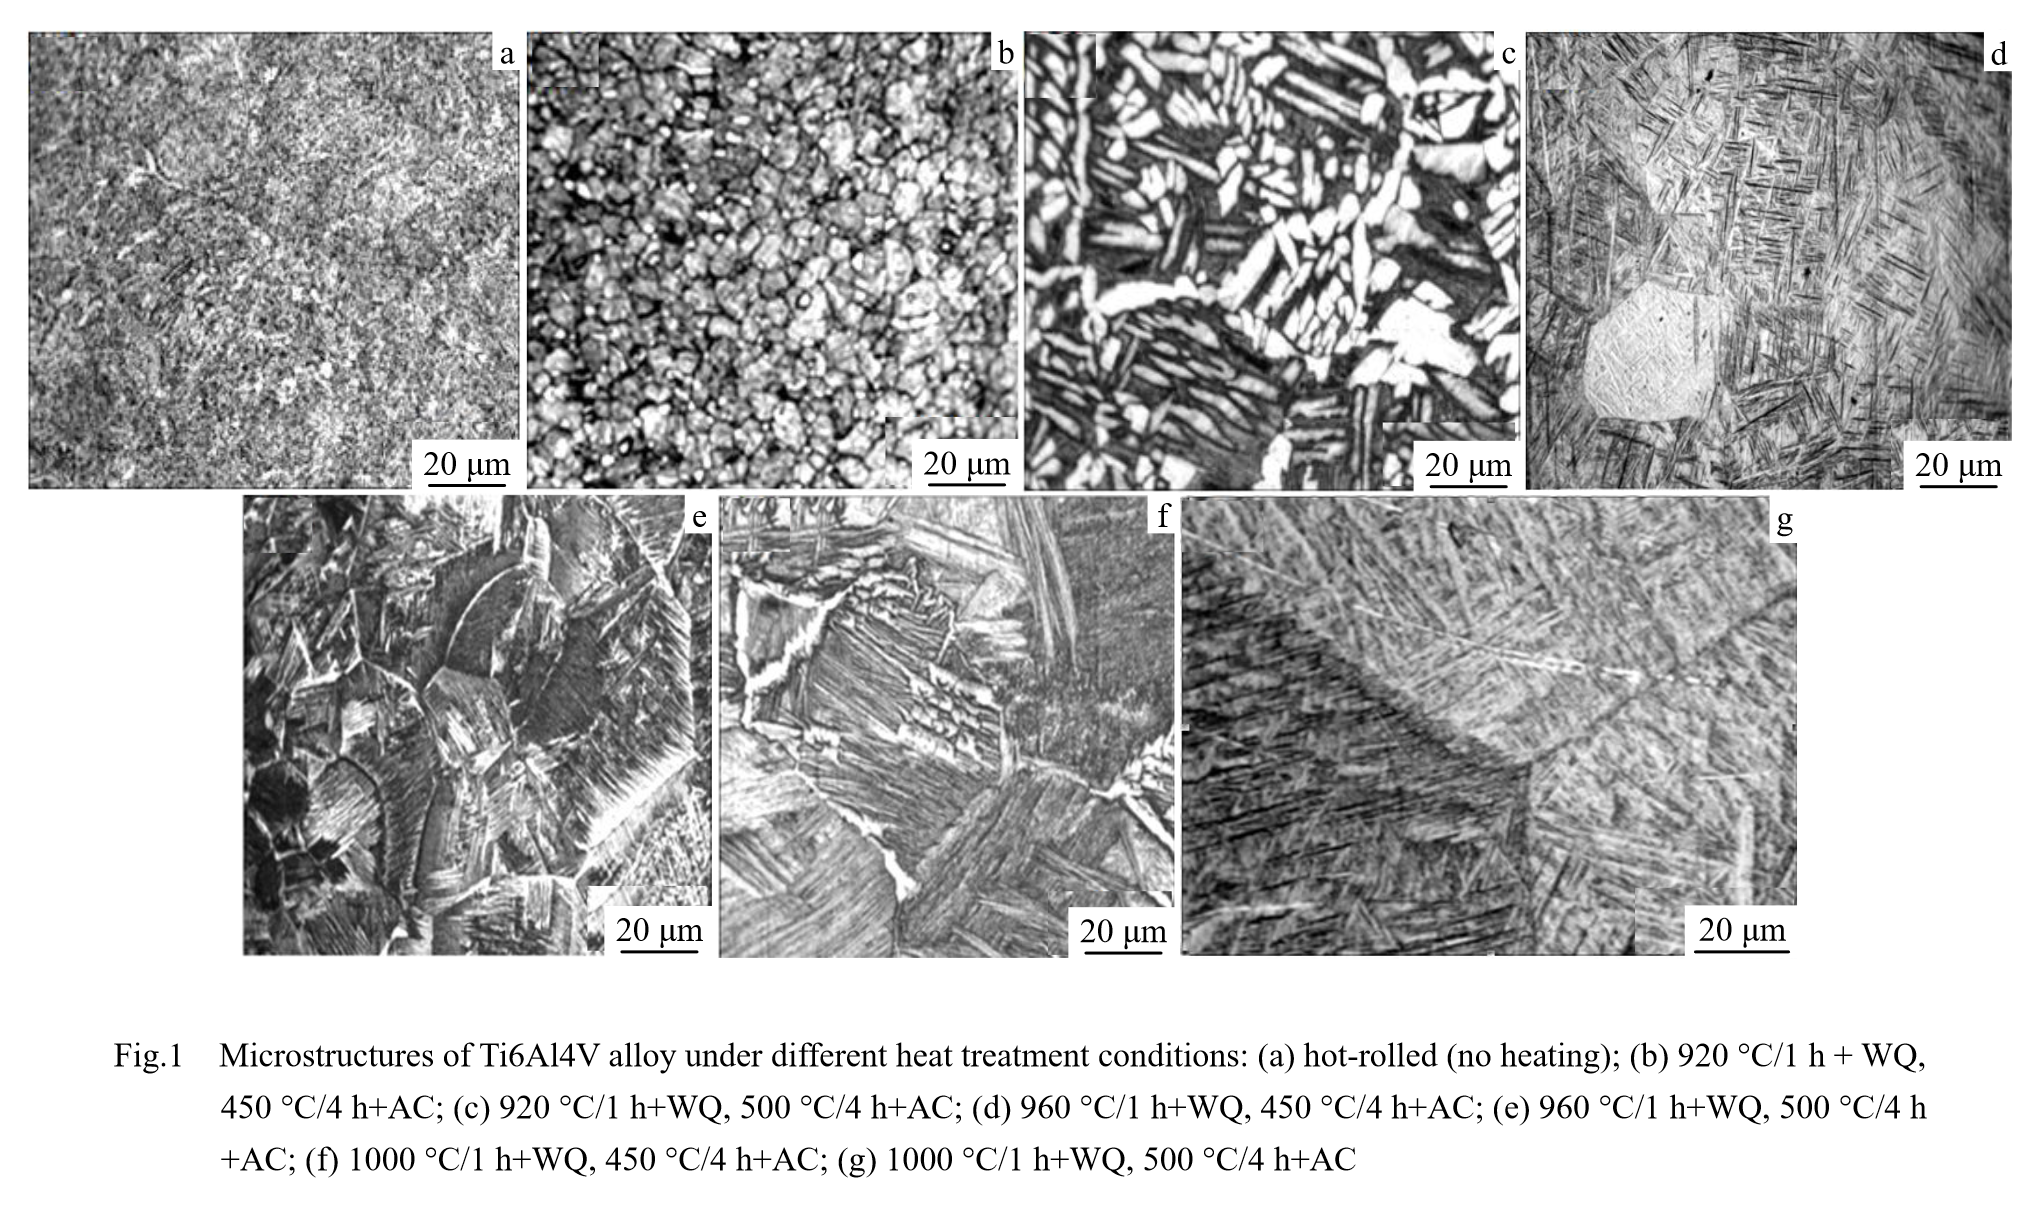
\includegraphics[width=0.8\linewidth]{金相_甲}
	\caption[参考一]{组织金相图}
	\label{fig:}
\end{figure}
% TODO: \usepackage{graphicx} required
\begin{figure}[h!]
	\centering
	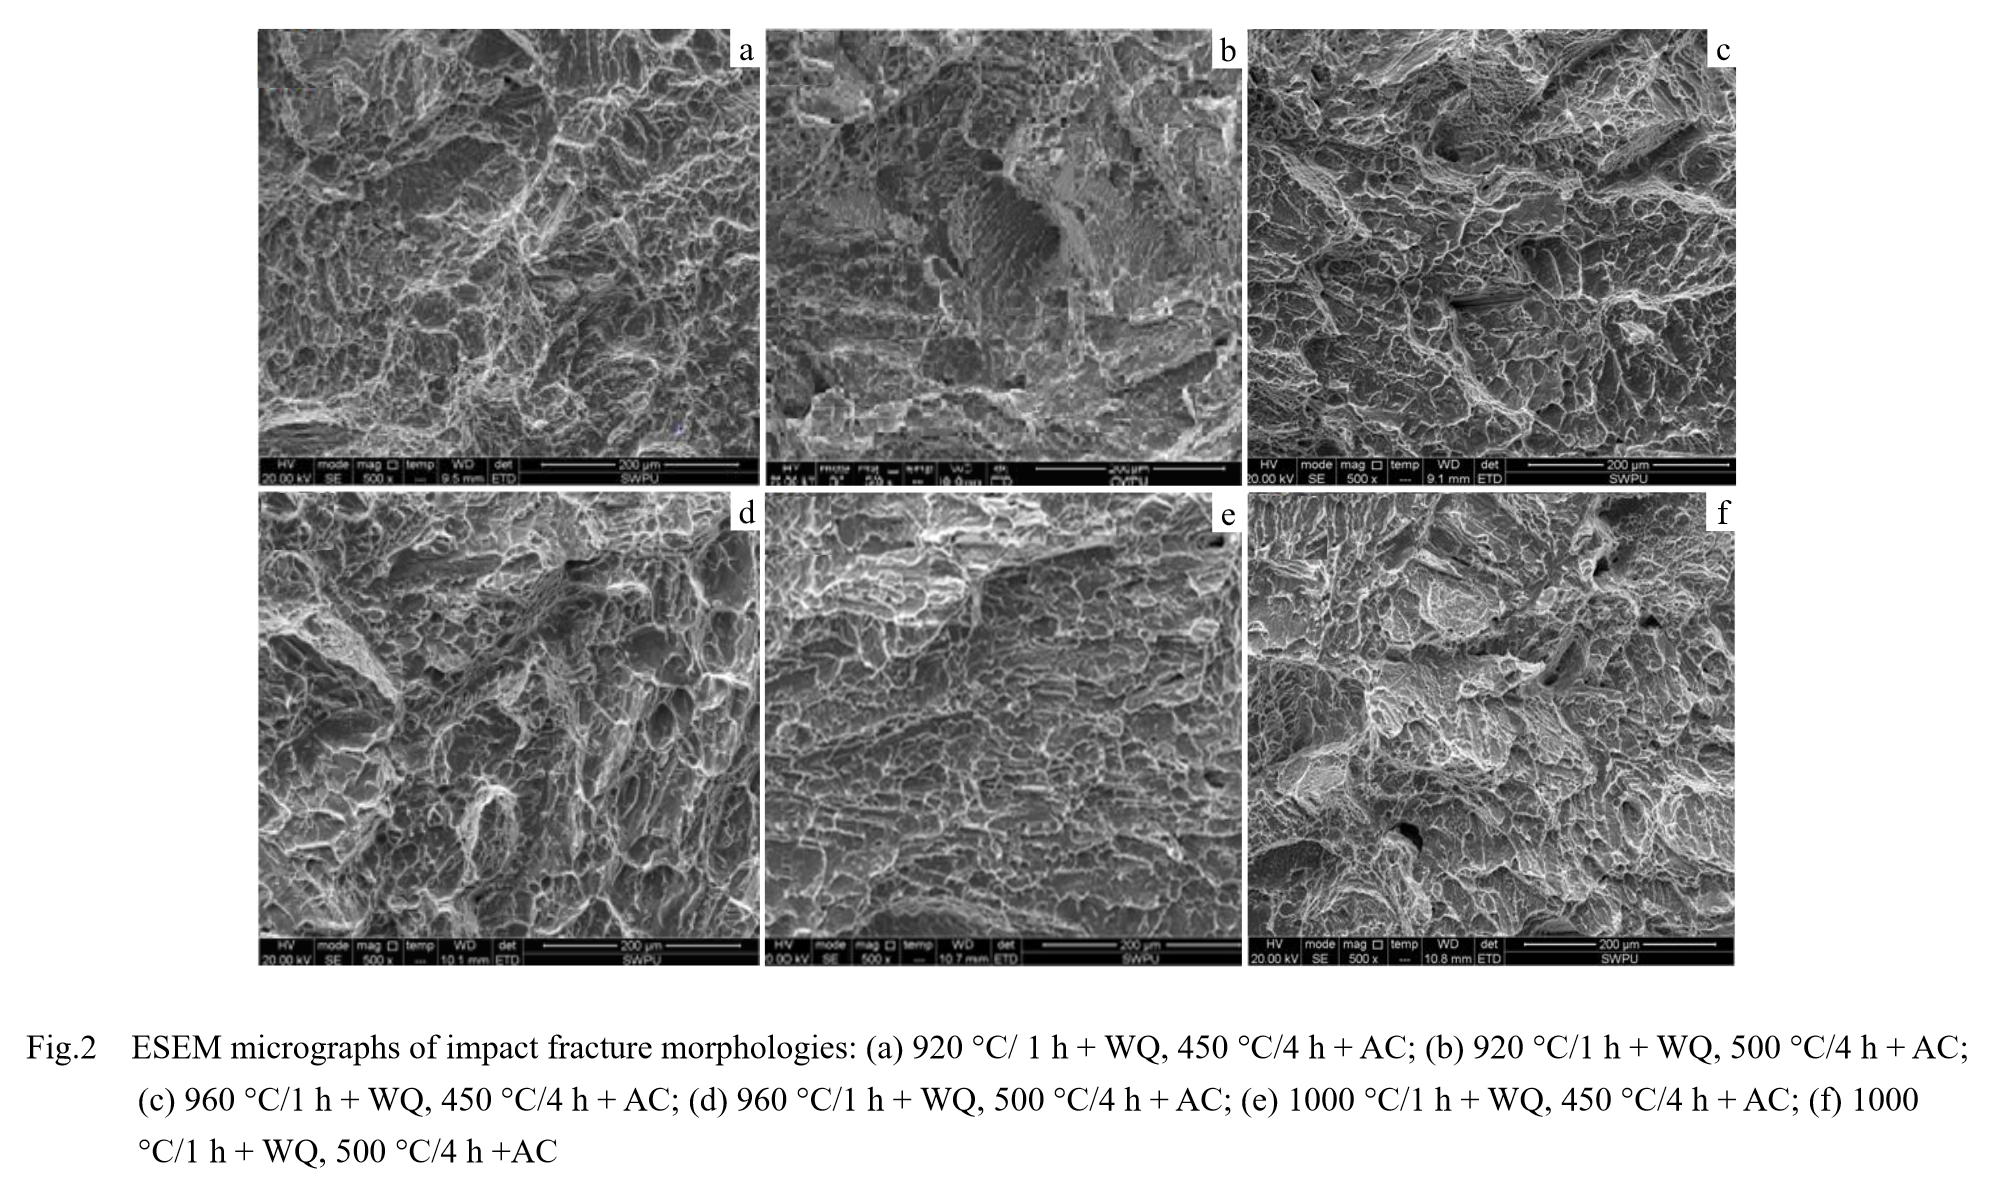
\includegraphics[width=0.8\linewidth]{其他_甲}
	\caption{断口形貌}
	\label{fig:}
\end{figure}